\documentclass[10pt,a4paper]{article}
\usepackage[latin1]{inputenc}
\usepackage{amsmath}
\usepackage{amsfonts}
\usepackage{amssymb}
\usepackage{graphicx}

\title{NetInf Service Specifications}

\begin{document}


\maketitle

\section{Components}

The frontend team's product consists of two Android applications:
\begin{enumerate}
\item NetInfService, providing a NetInf node.
\item A simple browser, henceforth called "Application", using NetInf through the NetInfService to cache and share web pages.
\end{enumerate}

\subsection{NetInfService}

The NetInfService provides a RESTful API that allows any application running on the same device as the NetInfService to access NetInf functionality through simple HTTP requests. The interface is described in detail in Section \ref{TODO ref interfaces}. NetInfService uses parts of OpenNetInf to provide this functionality. An overview of how the NetInfService works can be seen in Figure \ref{fig:netinfserviceoverview}.

\begin{figure}[h!]
	\centering
		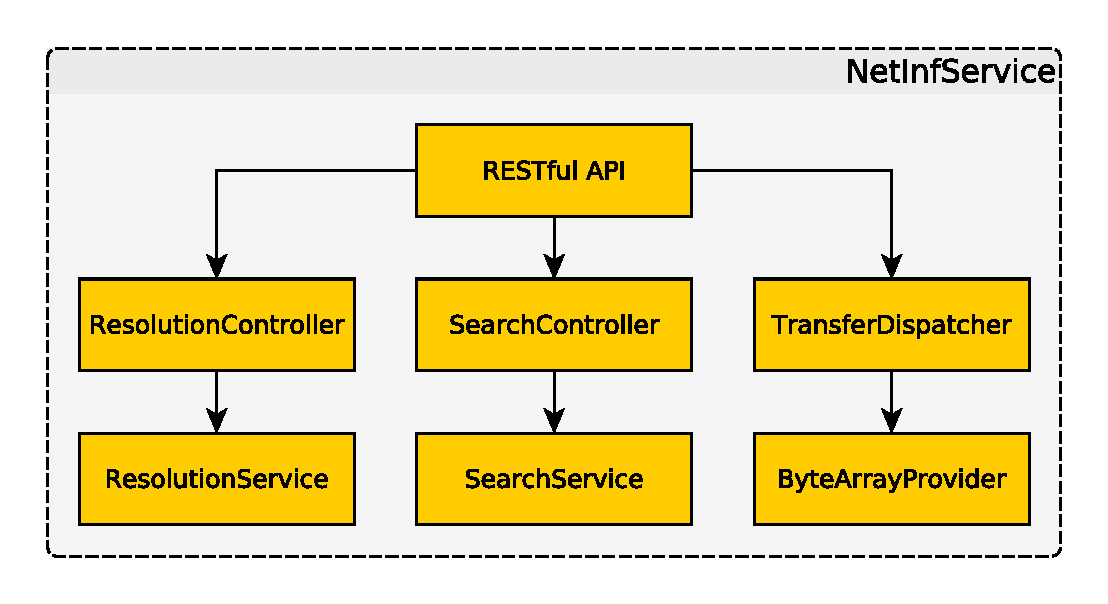
\includegraphics[width=0.75\textwidth]{netinfservice}
    	\caption{NetInfService Overview}
	\label{fig:netinfserviceoverview}
\end{figure}

\subsubsection{RESTful API}

The RESTful API receives HTTP requests. Depending on the type of request the ResolutionController, SearchController or TransferDispatcher is called. Publish requests are handled by the ResolutionController. Retrieve requests first do a get using the ResolutionController and then, if the get response contained locators, transfer the file using the TransferDispatcher. Search requests are handled by the SearchController.


\subsubsection{ResolutionController}

The ResolutionController handles a number of ResolutionServices. Each ResolutionServices should provide publish, get, and delete functionality using some convergence layer or equivalent. Currently there are two ResolutionServices. The LocalResolutionService which uses a local SQLite database and the NameResolutionService which communicates with a specific NRS using the HTTP convergence layer.

\subsubsection{SearchController}

The SearchController handles a number of SearchServices. Each SearchService should provide search functionality using some convergence layer or equivalent. Currently there is one SearchService. The UrlSearchService which provide search functionality using a single string which is assumed to be a URL.

\subsubsection{TransferDispatcher}

The TransferDispatcher handles a number of ByteArrayProviders. Each ByteArrayProvider should provide functionality to retrieve a file (as a ByteArray) in some way. Currently there is one ByteArrayProvider. The BluetoothProvider which uses Bluetooth to transfer files from other Bluetooth enabled devices.

\subsection{Application}

The idea behind the browser Application is simple. When a traditional web URL is entered into the address bar and you click the refresh button, instead of just downloading the webpage from the Internet the application first tries to use NetInf to retrieve the webpage.

This is done by using the NetInfService. For the entered URL and each resource it links to:
\begin{enumerate}
	\item Search for the hash of the URL/resource.
	\item Get the file with the given hash.
	\item Possibly publish the file so that others devices can get the file from this device.
\end{enumerate}

If the search or get fails for any reason, be it a timeout, no matches found or something else, the webpage is downloaded using the Internet.

\subsection{Control Flow}

Figure \ref{fig:controlflow} shows a more detailed picture of the control flow of the Application and NetInfService. The picture provides the packages and/or source files that are involved in different parts of the program, as well as some text and arrows describing the control flow.

The NetInfService mainly does its work by passing around Identifiers and InformationObjects (which encapsulates an Identifier).

An Identifier contains information about an InformationObject. The most important pieces of information in these applications are:
\begin{itemize}
\item Hash Algorithm
\item Hash
\item Content-Type
\item Metadata (as a JSON string)
\end{itemize}

InformationObjects can contain attributes. In these applications the only used attributes are locator attributes. More specifically locators pointing to other Bluetooth devices and locators pointing to the local file system.

\begin{figure}[h!]
	\centering
		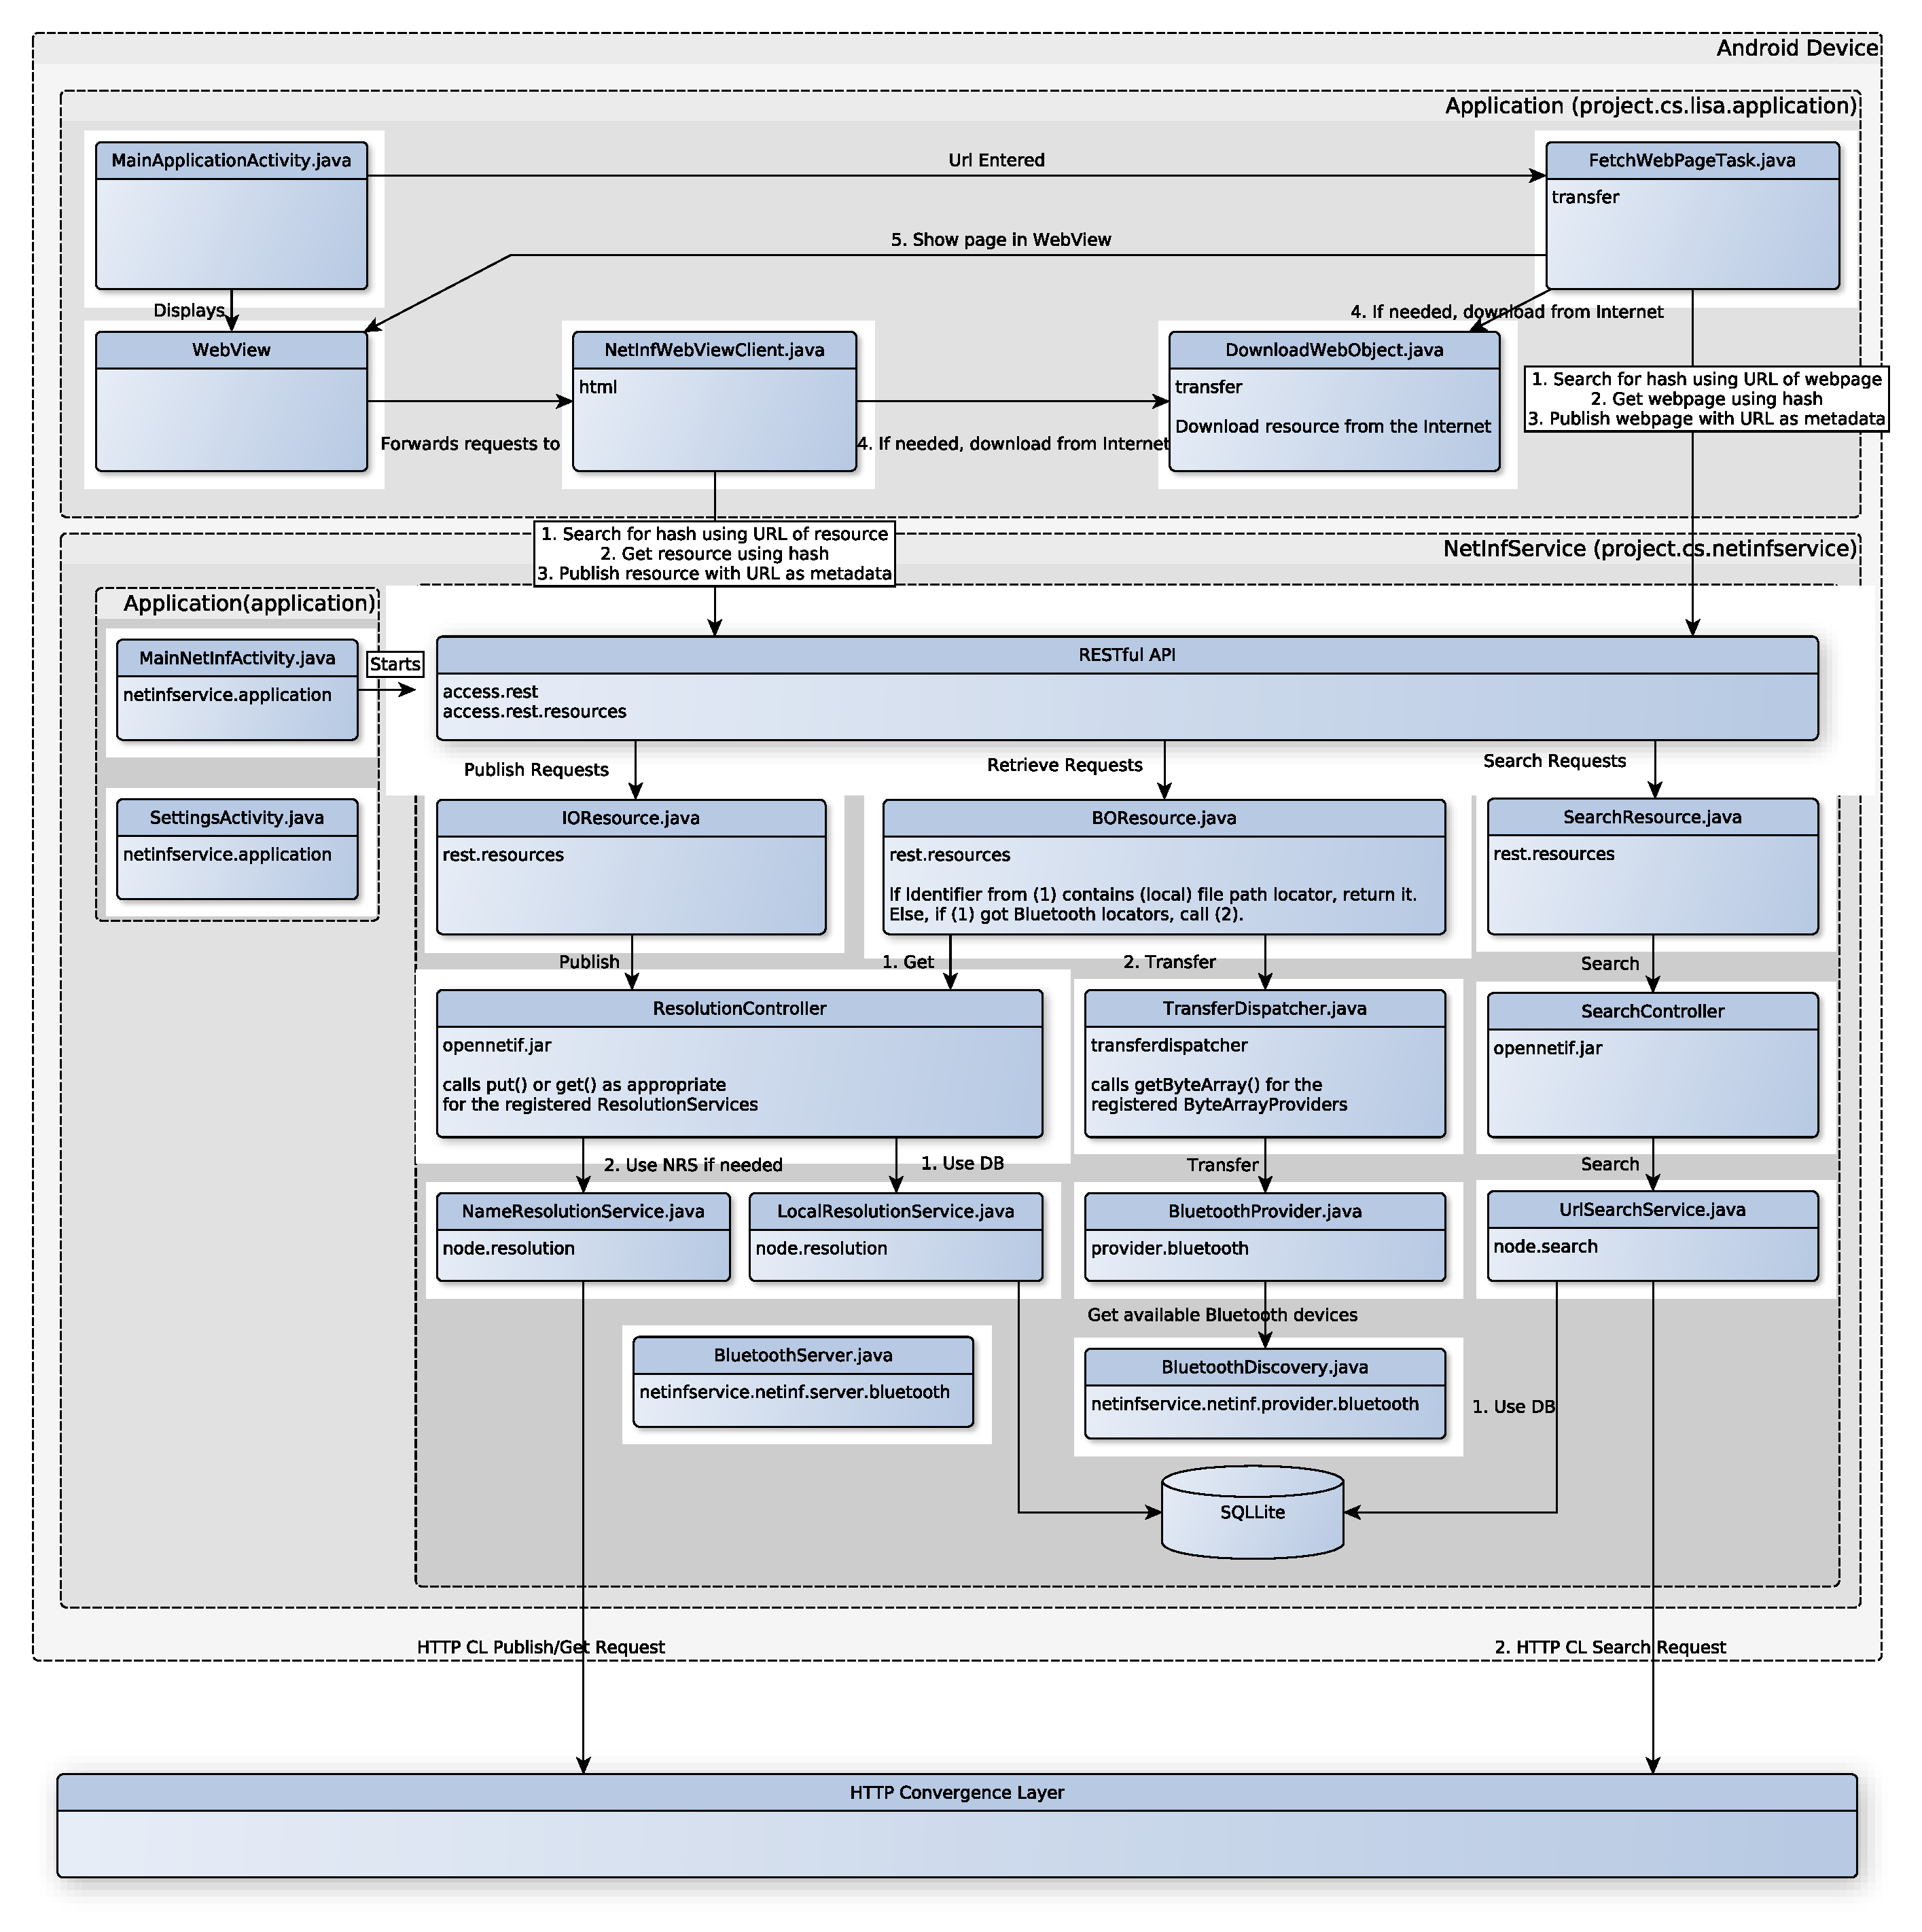
\includegraphics[width=1\textwidth]{flowchart}
    	\caption{Control Flow}
	\label{fig:controlflow}
\end{figure}

\section{HTTP RESTful Interface}
In order to communicate any application that wishes to use the NetInf service, there is a HTTP RESTful interface that can be used to 
send requests to the NetInf node. There is also a specification on what format this messages should have. In every message, regarding 
of the purpose of it, begins in the following way:\\


\begin{center}
http://\{Host\}:\{Port\}/\{Prefix\}?hash=\{Hash\}\&hashAlg=\{Hash Alg\}\\
\end{center}

Where:

\begin{itemize}
 \item Host: the IP address of the NetInf node. If the node is located in the same devices then the host could be \textit{localhost}.
 \item Port: the port of the NetInf node.
 \item Prefix: the name of the operation the application is requesting. 
 \item Hash: the hash of the object.
 \item Hash Alg: the hash algorithm used to hash the content e.g. sha-256
\end{itemize}

\subsection{Publish}
To publish a content, the prefix used is ``publish''. And the message will look like this:\\

\begin{center}
http://\{Host\}:\{Port\}/publish?\\
hash=\{Hash\}\&hashAlg=\{Hash Alg\}\&ct=\{Content Type\}\\
\&btmac=\{Bluetooth MAC Address\}\\
\&filepath=\{File Path\}\&meta=\{Meta-data\}\\
\end{center}

\begin{itemize}
 \item Content Type: The MIME content type of the object that is being publish.
 \item Bluetooth MAC Address: the MAC Address of the device, so it will be added as a locator.
 \item File Path: the file path of the object that is being published. This is used when a full put is done to the Name Resolution Service. In the case that the application
 does not want to do a full put then this field can be empty, ignoring also the header ``\&filepath=''.
 \item Meta-data: the meta-data for the object that is being published. The meta-data is a JSON object has to be encoded for URLs and it has the following format:\\
  \{meta\}:\{...\}\\
 \end{itemize}

\subsection{Retrieve}
To retrieve content, the prefix used is ``retrieve''. And the message should look like this:\\

\begin{center}
http://\{Host\}:\{Port\}/retrieve?hash=\{Hash\}\&hashAlg=\{Hash Alg\}\\\end{center}


\subsection{Search}
To search content the prefix used is ``search''. And the message contains tokens for the search:\\

\begin{center}
http://\{Host\}:\{Port\}/search?tokens=\{Tokens\}\&ext=\{Ext\}\\
\end{center}
Right now, the NetInf Service only supports one token and the ext field is not used although it has been defined to satisfy the NetInf specification.\\


\section{Installation}
The NetInf service runs as a regular Android application. It has to be installed either through Eclipse by running while the phone is connected to the computer 
or installing the .adk directly in the phone. It is important to have the NetInf service up and running for using any type of application that wants to communicate with it. \\


\section{Settings}
The NetInf service has a settings menu. There you can set the address and the port of the Name Resolution Service. Also, there is a Bluetooth Server switch that turns on 
and off the function of sharing objects through Bluetooth.\\

\end{document}